%!TEX TS-program = xelatex
\documentclass[a4paper]{friggeri-cv}
\usepackage{afterpage}
\usepackage{hyperref}
\usepackage{color}
%\usepackage{xcolor}
\usepackage{smartdiagram}


% if you want to add fontawesome package
% you need to compile the tex file with LuaLaTeX
% References:
%   http://texdoc.net/texmf-dist/doc/latex/fontawesome/fontawesome.pdf
%   https://www.ctan.org/tex-archive/fonts/fontawesome?lang=en
%\usepackage{fontawesome}
\usepackage{metalogo}
\usepackage{dtklogos}
\usepackage[utf8]{inputenc}
\usepackage{biblatex}
\usepackage{graphicx}
\usetikzlibrary{mindmap,shadows}
\hypersetup{
pdftitle={},
pdfauthor={},
pdfsubject={},
pdfkeywords={},
colorlinks=false,           % no lik border color
allbordercolors=white       % white border color for all
}
\smartdiagramset{
bubble center node font = \footnotesize,
bubble node font = \footnotesize,
% specifies the minimum size of the bubble center node
bubble center node size = 1.0cm,
%  specifies the minimum size of the bubbles
bubble node size = 0.5cm,
% specifies which is the distance among the bubble center node and the other bubbles
distance center/other bubbles = 0.3cm,
% sets the distance from the text to the border of the bubble center node
distance text center bubble = 0.5cm,
% set center bubble color
bubble center node color = pblue,
% define the list of colors usable in the diagram
set color list = {lightgray, materialcyan, orange, green, materialorange, materialteal, materialamber, materialindigo, materialgreen, materiallime},
% sets the opacity at which the bubbles are shown
bubble fill opacity = 0.6,
% sets the opacity at which the bubble text is shown
bubble text opacity = 0.5,
}

%\addbibresource{bibliography.bib}
\RequirePackage{xcolor}
\definecolor{pblue}{HTML}{0395DE}

\begin{document}
    \header{Ali}{Heydari}
    {Computer Engineer}

    % Fake text to add separator
    \fcolorbox{white}{gray}{\parbox{\dimexpr\textwidth-2\fboxsep-2\fboxrule}{%
    .....
    }}

    % In the aside, each new line forces a line break
    \begin{aside}
        \includegraphics[scale=0.037]{../assets/images/Ali_Heydari.jpg}
        \section{Address}\label{sec:address}
        Iran- Tehran- Narmak -
        Iran University of Science and Technology.
        ~
        \section{Tel \& Skype}\label{sec:tel&skype}
        \href{tel:+989368563509}{+98 936 856 3509}
        ~
        \section{Mail}\label{sec:mail}
        \href{mailto:ali4heydari@gmail.com}{\textbf{ali4heydari@}\\gmail.com}
        ~
        \section{Github}\label{sec:git}
        \href{https://github.com/ali4heydari}{github.com/ali4heydari}
        %\href{https://gitlab.com/u/ali4heydari}{gitlab.com/u/ali4heydari}
        %~
        % use  \hspace{} or \vspace{} to change bubble size, if needed
        \section{Programming}\label{sec:programming}
        
\includegraphics[scale=0.03]{../assets/images/logos/Java_logo.png} \textbf{Java}%
\includegraphics[scale=0.33]{../assets/images/stars/2stars.png}

        
\includegraphics[scale=0.0047]{../assets/images/logos/Android_logo.png} \textbf{Android}%
\includegraphics[scale=0.33]{../assets/images/stars/1stars.png}

        %\textbf{\LaTeX}%
\includegraphics[scale=0.33]{../assets/images/stars/3stars.png}

        \textbf{C\#}%
\includegraphics[scale=0.33]{../assets/images/stars/2stars.png}

        \textbf{C++}%
\includegraphics[scale=0.33]{../assets/images/stars/1stars.png}

        
\includegraphics[scale=0.0045]{../assets/images/logos/Python_logo.png} \textbf{Python}%
\includegraphics[scale=0.33]{../assets/images/stars/1stars.png}

        
\includegraphics[scale=0.008]{../assets/images/logos/SQL_logo.png} \textbf{SQL}%
\includegraphics[scale=0.33]{../assets/images/stars/1stars.png}

        \textbf{C}%
\includegraphics[scale=0.33]{../assets/images/stars/1stars.png}
        ~
        \section{Skills}\label{sec:skills}
        \smartdiagram[bubble diagram]{
        Design \\
        Pattern,
        Microsoft \\
        Office,
        Photoshop,
        
\includegraphics[scale=0.025]{../assets/images/logos/Git_logo.png}\textbf{Git} ,
        \textbf{\LaTeX},
        Unit \\
        Testing,
        \textbf{TDD}
        }
        ~
        \section{OS Preference}\label{sec:os-preference}
        \textbf{Windows}
\includegraphics[scale=0.33]{../assets/images/stars/5stars.png}
        \textbf{GNU/Linux}
\includegraphics[scale=0.33]{../assets/images/stars/3stars.png}
        %    \textbf{MacOS}
\includegraphics[scale=0.33]{../assets/images/stars/1stars.png}
        %    \textbf{Unix}
\includegraphics[scale=0.33]{../assets/images/stars/2stars.png}
        ~
        \section{Places Lived}\label{sec:places-lived}
        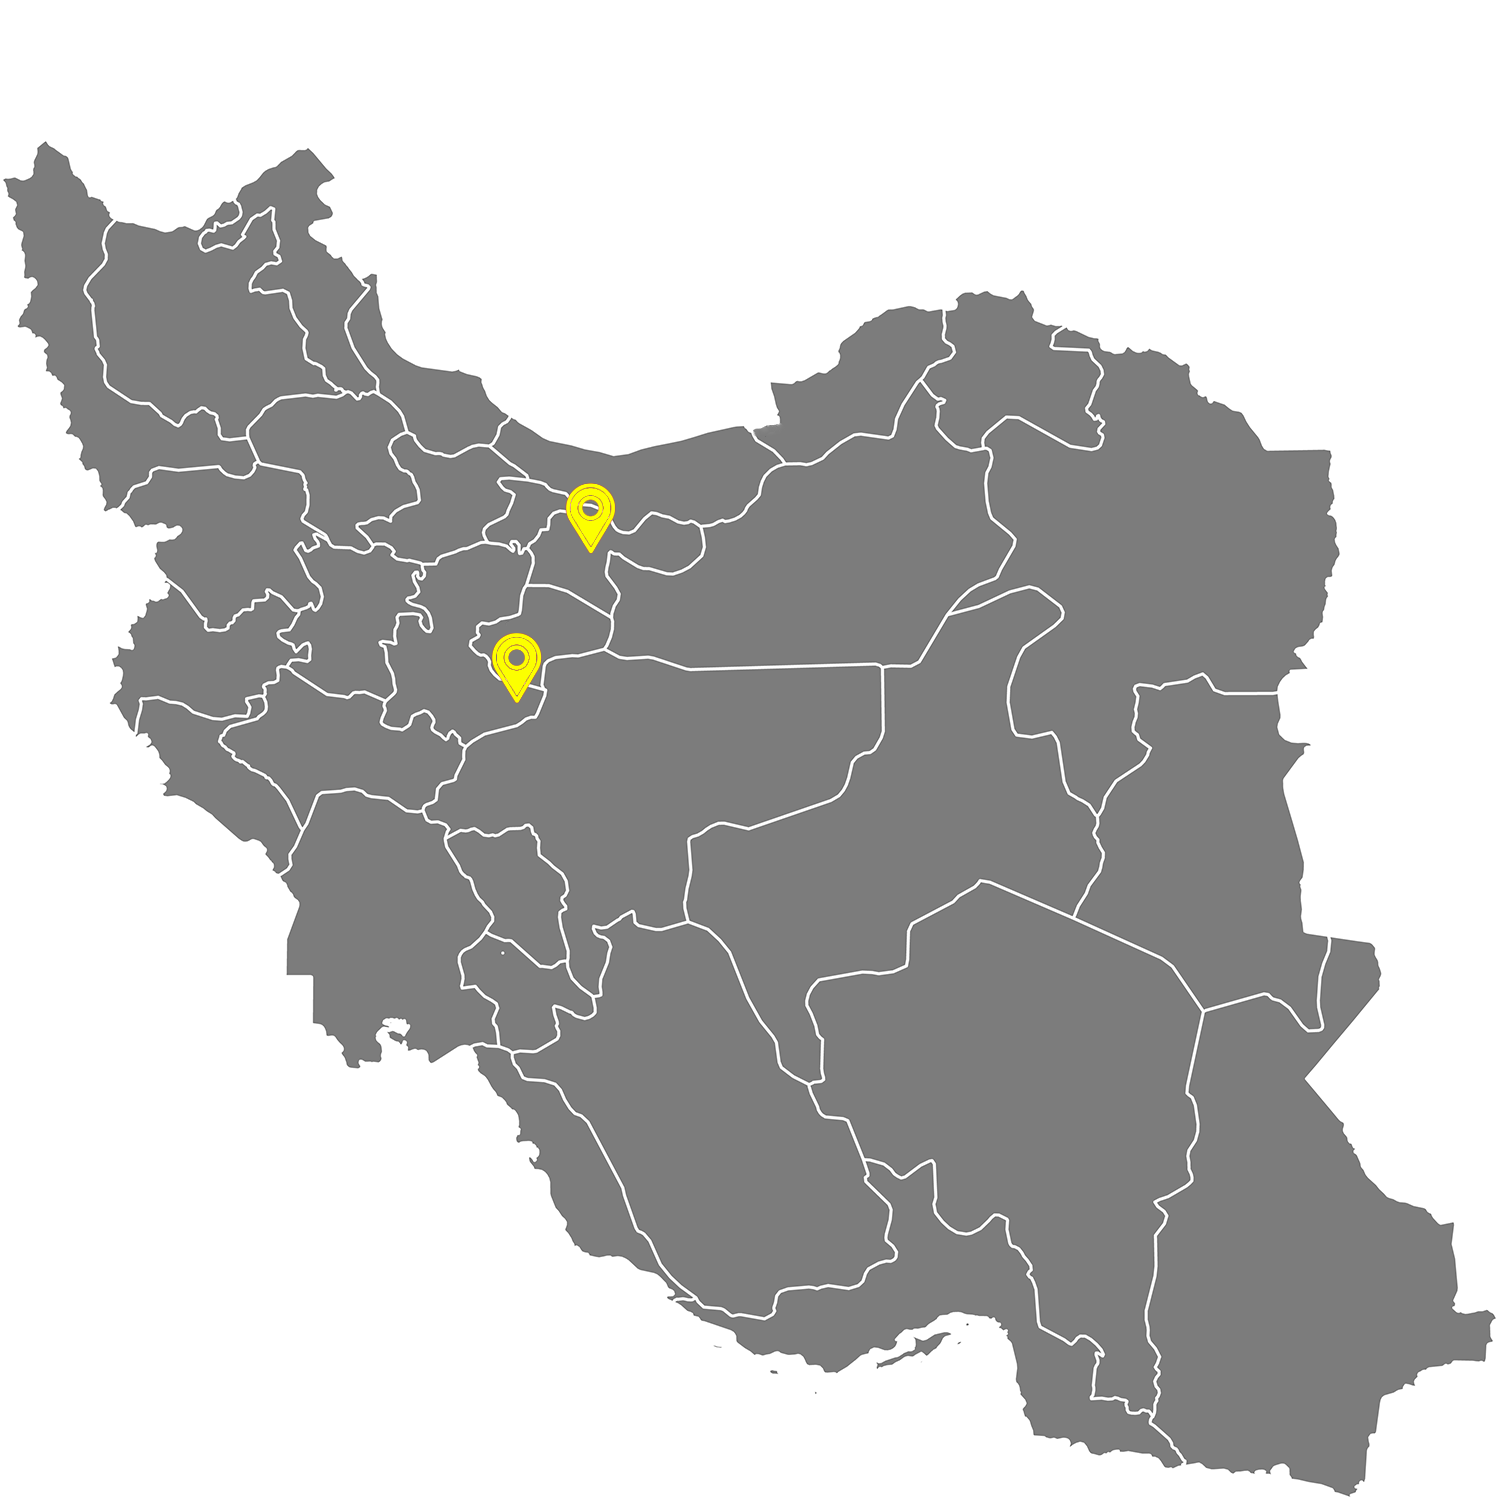
\includegraphics[scale=0.5]{../assets/images/iran.png}
        ~
        %   \section{Languages}
        % \textbf{Persian}
\includegraphics[scale=0.33]{../assets/images/stars/5stars.png}
        % \textbf{English}
\includegraphics[scale=0.33]{../assets/images/stars/2stars.png}
        % ~
    \end{aside}
    ~
    \section{Experience}\label{sec:experience}
    \begin{entrylist}
        \entry
        {01/18-07/18}
        {    Software developer}
        {\href{http://www.amngostar-co.com/}{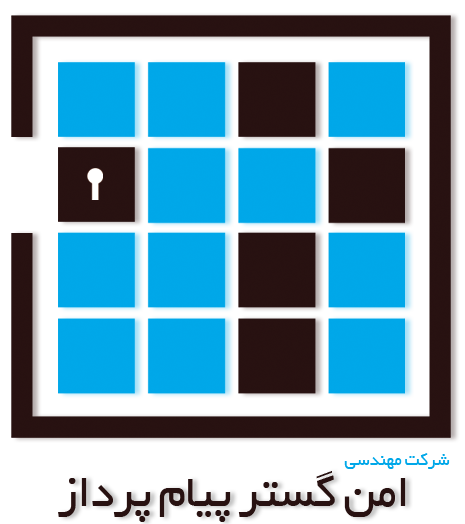
\includegraphics[scale=0.04]{../assets/images/logos/AmnGostar_logo.png} AmnGostar Co}}
        {Part-time software developer for \emph{Sepehr} ISMS software project}
        \entry
        {10/17-04/18}
        {    Teacher \& course officer}
        {\href{http://www.kanoon.ir/}{
\includegraphics[scale=0.005]{../assets/images/logos/Kanoon_logo.png} Kanoon Farhangi Amoozesh}}
        {Part-time teacher \& course officer of physics and mathematics courses}
        %\entry
        %{09/17-07/17}
        %{   \emph{Tabesh} Cultural Group}
        %{\href{http://www.sharif.ir/}{
\includegraphics[scale=0.03]{../assets/images/logos/Tabesh_logo.jpg} Sharif University of Technology}}
        %{Member of the \emph{Tabesh} Cultural Group}
        %\entry
        %{09/17-07/17}
        %{   Kimia Student Practical Group}
        %{\href{http://www.sharif.ir/}{
\includegraphics[scale=0.03]{../assets/images/logos/Kimia_logo.jpg} Sharif University of Technology}}
        %{Member of the \emph{Kimia} Student Practical Group}
        \entry
        {02/11-02/11}
        {    Calligraphy exhibition \emph{Noghte}}
        {\href{http://calligraphers.ir/}{
\includegraphics[scale=0.15]{../assets/images/logos/Khoshnevisan_logo.png}Association of the Calligraphers of Delijan}}
        {Participation in calligraphy exhibition \emph{Noghte}}
        \entry
        {02/08-06/10}
        {   Calligrapher}
        {\href{http://calligraphers.ir/}{
\includegraphics[scale=0.15]{../assets/images/logos/Khoshnevisan_logo.png}Association of the Calligraphers}}
        {Member of association of Calligraphers of Delijan}
    \end{entrylist}
    \\
    \section{Education}\label{sec:education}
    \begin{entrylist}
        \entry
        {2017 - Now}
        {     B.Sc in Computer Engineering}
        {\href{http://www.iust.ac.ir/}{
\includegraphics[scale=0.08]{../assets/images/logos/IUST_logo_color.png}Iran University of Science and Technology}}
        {}

        \entry
        {2016 - 2017}
        {    B.Sc in Chemical Engineering (Unfinished)}
        {\href{http://www.sharif.ir/}{
\includegraphics[scale=0.015]{../assets/images/logos/Sharif_logo.png} Sharif University of Technology}}
        {}

        \entry
        {2011 - 2015}
        {    Scientific Diploma}
        {Beheshti Highschool}
        {}
    \end{entrylist}

    %\newpage

    \section{Honors \& Awards}\label{sec:honors&awards}
    \begin{entrylist}

        %             \entry
        %    {06/2014}
        %    {   441 rank}
        %    {Competitive examination}
        %    {441 rank at the National Maths-Physics competitive examination}

        \entry
        {06/2014}
        {Kharazmi Festival rank}
        {\href{http://kharazmi.medu.ir/fa/}{
\includegraphics[scale=0.06]{../assets/images/logos/YKharazmi_logo.jpg} Iran Kharazmi Festival}}
        {The first rank in the provincial section and the country's highest rank}

        \entry
        {03/2014}
        {   Invention of \emph{Damaban SAMA}}
        {\href{http://iripo.ssaa.ir/}{
\includegraphics[scale=0.06]{../assets/images/logos/Ghovveh_logo.jpg} Iranian Patent Office}}
        {Holds a patent for \\
        invention of \emph{Damaban SAMA}}

        \entry
        {04/2013}
        {   Invention of \emph{Ghalamgir khoshnevisi}}
        {\href{http://iripo.ssaa.ir/}{
\includegraphics[scale=0.06]{../assets/images/logos/Ghovveh_logo.jpg} Iranian Patent Office}}
        {Holds a patent for\\
        invention of \emph{Ghalamgir khoshnevisi}}

    \end{entrylist}
    \section{Certifications}\label{sec:certifications}
    \begin{entrylist}
        \entry
        {08/2018}
        {Software design patterns}
        {\href{http://coursera.org/}{
\includegraphics[scale=0.08]{../assets/images/logos/Coursera_logo.jpg} Coursera} - by \href{https://www.ualberta.ca/}{
\includegraphics[scale=0.05]{../assets/images/logos/UAlberta_logo.jpg} University of Alberta}}
        {}

        \entry
        {02/2013}
        {Calligraphy \emph{Momtaz} Degree}
        {\href{http://calligraphers.ir/}{
\includegraphics[scale=0.15]{../assets/images/logos/Khoshnevisan_logo.png}Iran Calligraphers Association}}
        {}

        \entry
        {02/2014}
        {Invention Authorization for \emph{Damaban SAMA}}
        {\href{http://www.irost.org/}{
\includegraphics[scale=0.09]{../assets/images/logos/IROST_logo.jpg} IROST}}
        {}

    \end{entrylist}
    \section{Skills}
    \smartdiagram[bubble diagram]{
    \textbf{Skills},
    Microsoft \\
    Office,
    Photoshop,
    
\includegraphics[scale=0.025]{../assets/images/logos/Git_logo.png}\textbf{Git} ,
    \textbf{\LaTeX},
    \textbf{TDD},
    }
    %\begin{flushleft}
    %\emph{August  2018}
    %\end{flushleft}
    %\begin{flushright}
    %\emph{Ali Heydari}
    %\end{flushright}

\end{document}
